\documentclass[a4paper]{article}

%%%%% Paquetes

\usepackage[spanish]{babel} 
\usepackage[utf8]{inputenc}
\usepackage{makeidx} %Indice
\usepackage{amsmath} %Ecuaciones sin numero al costado
\usepackage{graphicx} %Imagenes
\usepackage{fancyhdr} %Para encabezado y pie de pagina
\usepackage{float} %Para forzar la posicion de la imagen
\usepackage[hidelinks]{hyperref} %Para url y links
\hypersetup{colorlinks=false}

\usepackage{longtable} %Para tablas que ocupan mas de una hoja

% Para las notas al pie dentro de tablas o tabulaciones
\usepackage{tablefootnote}

%%%%% Paquetes

\begin{document}

\pagenumbering{gobble} %No numerar la primer pagina

\begin{titlepage}
	\centering
	
\includegraphics{Imagenes/logo_fiuba.png}\par\vspace{1cm}
	{\scshape\LARGE Facultad de Ingeniería \par
	Universidad de Buenos Aires  \par}
	\vspace{1.5cm}
	{\Large\bfseries Trabajo Profesional de Ingeniería en Informática\par}
	\vspace{1.5cm}
	{\huge\bfseries MUSSA \par}
	\vspace{0.5cm}
	{\huge\bfseries Generador de Planes de Carrera personalizados\par}
	\vspace{1cm}
	{\Large\itshape Jennifer Andrea Woites\par}
	\vfill
	{\Large
	Tutor: Lic. Rosa Wachenchauzer \par
	\vspace{0.3cm}
	Co-Tutor: Ing. Diego Essaya}
	\vfill
% Bottom of the page
	{\large Abril, 2018 \par}
\end{titlepage}

  \newpage
  
  \pagenumbering{arabic} %Comenzar a numerar las paginas

  \tableofcontents % Indice
    
%%%% Cabecera y pie de pagina
  \pagestyle{fancy}
  \lhead{Jennifer Andrea Woites - Padrón: 93274}
  \rhead{}
  \renewcommand{\headrulewidth}{0.4pt} % grosor de la línea de la cabecera
%%%% Cabecera y pie de pagina

  \newpage


\section{Introducción}

El siguiente documento presenta el Trabajo Profesional de Ingeniería en Informática de la estudiante Jennifer Andrea Woites, padrón 93274. Los docentes que estuvieron a cargo son: Lic. Rosa Graciela Wachenchauzer como tutora del trabajo profesional, y el Ing. Diego Essaya como cotutor. \newline

El objetivo del proyecto es aplicar los conocimientos adquiridos en la carrera. \newline

El tema del trabajo profesional es <<MUSSA\footnote{Materias Universitarias en un Sistema Simplificado Automático} - Generador de Planes de Carrera personalizados.>> \newline

El objetivo general del presente trabajo, es la realización de una web responsive que permita a los alumnos la visualización de sus materias, la administración de las mismas, la utilización de encuestas y la generación de un plan de carrera en base a parámetros personalizados, siendo ésto último el ítem más importante del trabajo.

\subsection{Motivación}

Durante los años en que el alumno lleva adelante la carrera, muchas veces se ve obligado a no seguir con las materias tal como figuran en el plan por diversos motivos: cupos llenos en las cursos que prefiere, decisión para cursar con otros compañeros, necesidad de cursar menos materias por cuatrimestre, incompatibilidad laboral, razones personales, etc. Estos alumnos se ven forzados a tener que rediseñar el plan para poder acomodar las materias en un tiempo razonable de realización, que además sea compatible con las preferencias que él o ella tengan.

A esto, se suman materias que solo se dictan en el primer o segundo cuatrimestre, las correlatividades, entre otras, que dificultan la decisión de qué materia realizar antes que otra.

Luego, se debe tener en cuenta que en muchos de los planes de estudio, las materias electivas no están clasificadas por ramas o intereses y que es parte de las decisiones que debe tomar el alumno el elegir qué materias desea cursar, muchas veces decidiendo más por el nombre que por el contenido en sí porque no necesariamente sabe si le está aportando conocimiento en el área a la que le gustaría dedicarse. En otros casos, por comentarios de algunos compañeros que previamente cursaron dichas materias, es capaz de asesorarse y decidir con un razonamiento más amplio.

Actualmente, la decisión de qué materia se cursa primero y cuál después, se toma "manualmente", es decir, se observa el punto en el que se está parado y se decide en base a lo mejor que se puede hacer en el corto plazo ya que es muy difícil observar el panorama completo cuanto más lejos de la meta se está.

En el marco de re inserción de alumnos que han abandonado la carrera y que le restan pocas materias por recibirse, es útil poder contar con una herramienta que priorice las materias en base a los tiempos que esta persona tiene disponible y tratar de recomendarle los mejores cursos para que pueda recibirse con prontitud, de forma de poder incrementar el número de profesionales recibidos en Argentina.

Se busca entonces, poder facilitar estas tareas a través de una plataforma web que permita obtener la información requerida para clasificar las materias (por ejemplo, a través de las encuestas), que facilite la generación de las notas para trámites como pedidos de créditos o excepciones de correlatividades que han de presentarse en la facultad posteriormente, y que, a través de parámetros configurados por el usuario, pueda armar automáticamente un plan de carrera que se ajuste a sus necesidades, pudiendo ser mutado si las mismas cambian con el paso del tiempo.

\section{Alcance}

El alcance del trabajo es:

\begin{enumerate}
	\item Desarrollar una página web responsive que conste de los siguientes:
		\begin{itemize}
			\item Login / Sign In / Cambio de Contraseña
			\item Almacenamiento y edición de datos personales, carreras, materias aprobadas / desaprobadas / con final pendiente / en curso
			\item Materias habilitadas para cursar
			\item Formularios: Nota al decano y listado de materias
			\item Encuestas de cursos / docentes
			\item Busquedas de materias con filtros
			\item Visualizar y Generar Plan de Estudios
		\end{itemize}

	\item Permitir la administración desde la web:
		\begin{itemize}
			\item Cursos
			\item Docentes
			\item Carga de horarios desde PDF
		\end{itemize}
		
	\item Modelar y desarrollar el algoritmo para la generación del plan de estudios personalizada
\end{enumerate}

\section{Tecnologías y Herramientas}

A continuación se detallan las herramientas y tecnologías más importantes que fueron utilizadas durante el desarrollo del trabajo.\newline

Como entorno de desarrollo se había elegido Sublime, pero posteriormente se cambió a Intellij IDEA ya que proveía de el debugger incorporado y otras funcionalidades básicas que no estaban disponibles en Sublime.\newline

Para el control de versiones fue utilizado GitHub\footnote{El proyecto MUSSA se encuentra en \url{https://github.com/jennywoites/MUSSA}}.\newline

Para la administración del proyecto se utilizó GDocs y Trello.\newline

Para la generación de documentación, tanto de la propuesta como del presente informe se utilizó Latex.\newline

Se eligió como lenguaje Python junto a Flask\footnote{http://flask.pocoo.org/} para el backend. Flask fue elegido a pesar de no tener experiencia por estar escrito en Python y ser un framework minimalista con una curva de aprendizaje relativamente rápida.\newline

El frontend fue desarrollado con HTML5, JavaScript, CSS y Bootstrap para que sea responsive.\newline

Para la base de datos se eligió MySQL\footnote{https://www.mysql.com/}. Además fue utilizado SQLAlchemy\footnote{Python SQL toolkit and Object Relational Mapper - \url{https://www.sqlalchemy.org/}} como ORM\footnote{ORM: Object Relational Mapper. Un ORM simplifica el acceso a una base de datos por parte del programador convirtiendo toda sentencia sql a operaciones con objetos.}.\newline

La máquina con la que fueron realizadas las pruebas tiene las siguientes características:
XXXXXXXXXXXXXXXXXXXXXXXXXXXXXXXXXXXXXXXXXXXXXXXXXXXXXXXXXXXXXXXXXXXXXXXXXXXXXXXXXXXXXXXXXXXXXXXXXXXXXXXXXXXX
por lo que los tiempos de los algoritmos de generación del plan podrían mejorar si se tuviese una máquina con mejores características.\newline

Para el comienzo del proyecto se utilizó Flask-User\footnote{\url{https://github.com/lingthio/Flask-User}}. Este proyecto ofrece una estructura inicial con las acciones básicas de login/signin y manejo de contraseñas. Fue dicifil de configurar al principio ya que no se tenía experiencia con Flask en general, pero una vez configurado solo hizo falta realizar las customizaciones correspondientes. El problema principal que se tuvo al utilizar Flask-User en lugar de haber realizado los servicios manualmente es que cuando se quiso desarrollar la API no se la pudo independizar completamente del proyecto ya que sino, requería solucionar el cross domain o realizar una autenticación en ambos puntos. Como punto a favor es que simplificó mucho el desarrollo de esa sección y que proveyó de una estructura básica al proyecto en general.\newline

Para poder realizar los planes de forma asincónica, se utilizó Celery\footnote{Celery es una cola de tareas asincónica open source basada en el pasaje de mensajes distribuido - \url{http://www.celeryproject.org/}} para la cola de tareas asincónica junto a Redis\footnote{Redis es un almacén de estructura de datos de valores de clave en memoria rápido y de código abierto - \url{https://redis.io/}} como estructura para los datos de las tareas.\newline

Para la generación del plan con el algoritmo de programación lineal entera, se utilizó PuLP\footnote{\url{https://pythonhosted.org/PuLP/}}. PuLP es una librería Open Source escrita en Python. Es usada para describir problemas de optimización como modelos matemáticos. PuLP puede llamar a numerosos solvers de programación lineal, tales como CBC, GLPK, CPLEX, Gurobi, etc, para resolver el modelo y luego utilizar comandos de Python para manipular y mostrar el resultado de la solución. Durante el desarrollo del algoritmo se probaron diferentes solvers, pero finalmente fue elegido CBC ya que fue el que mejor repsondía en tiempos para el algoritmo ejecutado además de ofrecer multi-threading para la resolución del problema.

\newpage
\section{Página Web MUSSA: Acceso Público}

\subsection{Carreras y materias de la facultad}

Las diferentes carreras de la facultad están compuestas por una serie de materias obligatorias, posibilidad de un idioma obligatorio, posibilidad de rendir un examen de suficiencia de idioma, materias electivas, trabajo profesional, tesis, etc.

Para esta primer implementación se cargaron y modelaron los planes de estudios de Ingeniería en Informática y Licenciatura en Análisis de Sistemas (1986, plan `viejo'). Posteriormente en futuras implementaciones, se añadirán las carreras restantes.\newline

Cada materia tiene como datos su código, el nombre, los diferentes cursos disponibles con sus docentes y horarios, la cantidad de créditos y sus correlatividades.

Los horarios de los cursos de las materias mantienen un histórico, y se agrega una nota visual en caso de que sea un curso nuevo (en cuyo caso se repiten los horarios del cuatrimestre actual para el cuatrimestre faltante). Para cada curso de la materia, se indica si se dicta el 1º cuatrimestre, el 2º o ambos. Los cursos que no se dicten ningun cuatrimestre ya no serán mostrados en la oferta horaria, pero quedarán disponibles para que el administrador los pueda volver a habilitar.

Se decidió que cada materia de las diferentes carreras sea tratada como un objeto diferente por más que compartan el código, ya que lo más usual es que las correlativas sean diferentes, que una sea obligatoria de una carrera y de la otra sea electiva y a veces que no todos los cursos estén disponibles para ambas.

Los cursos en cambio, se modelarán como uno solo para el mismo código y se indicará las carreras para las que se encuentra habilitado. En el caso de los cursos que dictan diferentes códigos de materias en el mismo horario, serán tratados como cursos independientes.

Los docentes podrán estar vinculados a uno o más cursos.\newline

Desde el acceso público, se podrán hacer búsquedas de materias, búsquedas de docentes, ver algunos links útiles e información de las comisiones por carrera y los datos de contacto del proyecto en caso de que quieran hacer aportes al proyecto.\newline

\begin{figure}[H]
\centering
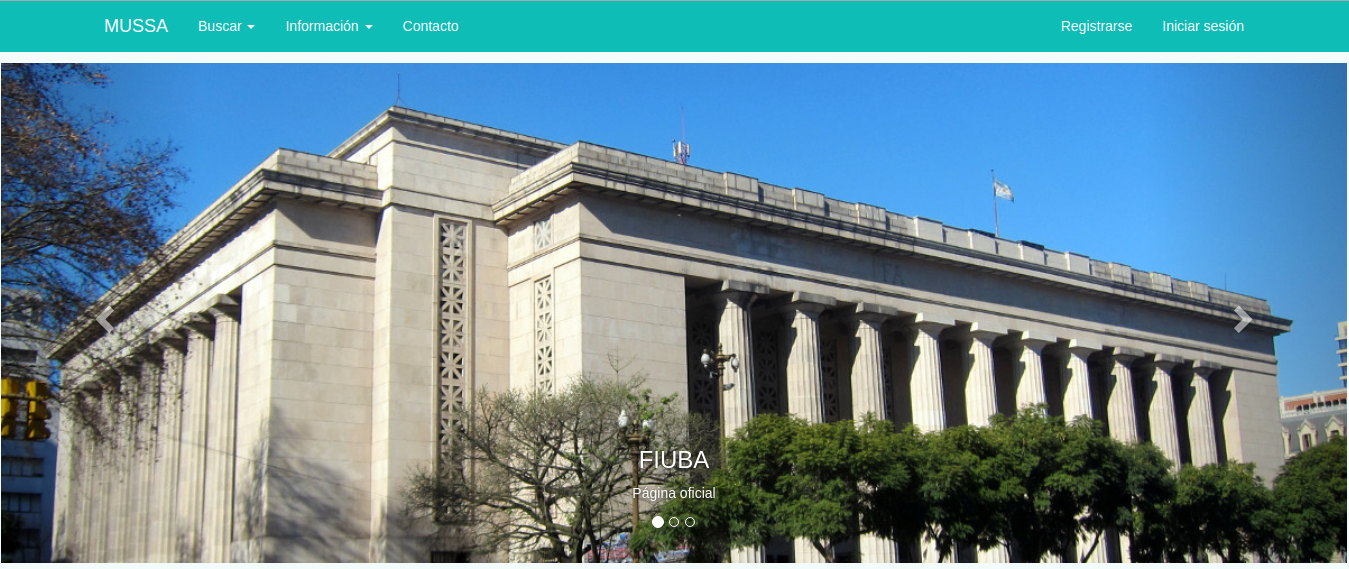
\includegraphics[scale=0.25]{Imagenes/pagina_inicio.png}\par
\caption{Página Inicio de MUSSA}
\end{figure}

\begin{figure}[H]
\centering
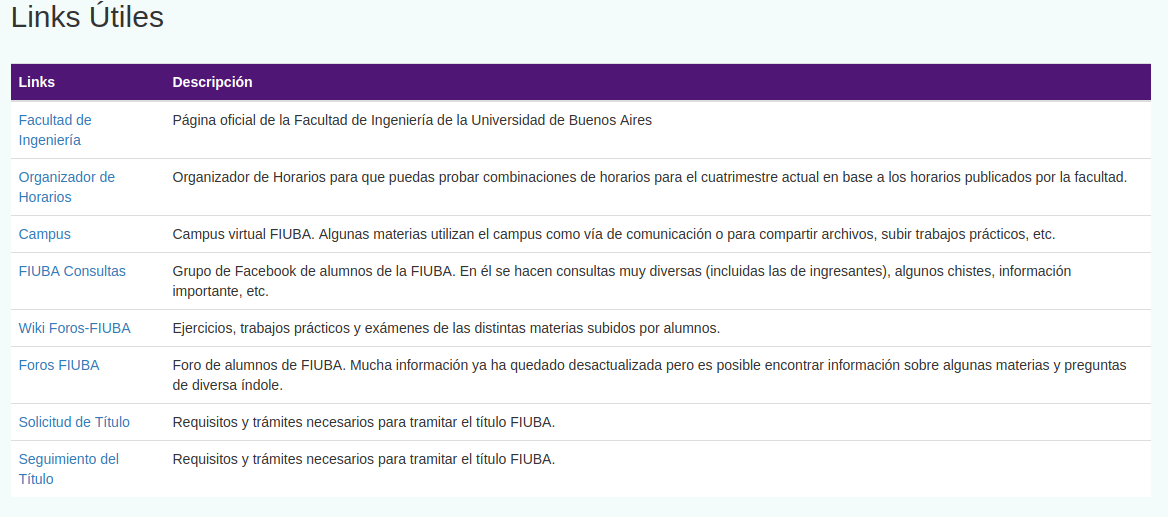
\includegraphics[scale=0.3]{Imagenes/links_utiles.png}\par
\caption{Links Útiles}
\end{figure}

\begin{figure}[H]
\centering
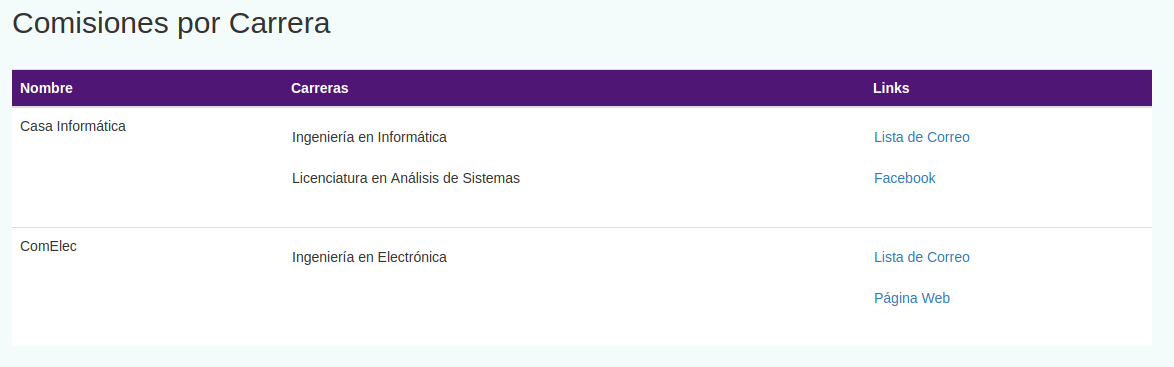
\includegraphics[scale=0.3]{Imagenes/comisiones.png}\par
\caption{Comisiones por carrera}
\end{figure}

\subsection{Búsqueda de Docentes}

La búsqueda de docentes se realiza buscando por parte del apellido o parte del nombre (no requiere que comience con las letras indicadas sino que éstas se encuentren en el campo indicado).

Como resultado se listarán todos los docentes que cumplan con el criterio de búsqueda. Para ellos, se podrá visualizar el nombre (si lo tienen) y el apellido, además de las materias que dicta. Luego, desde allí se puede acceder a las encuestas asociadas a éste docente.

\begin{figure}[H]
\centering
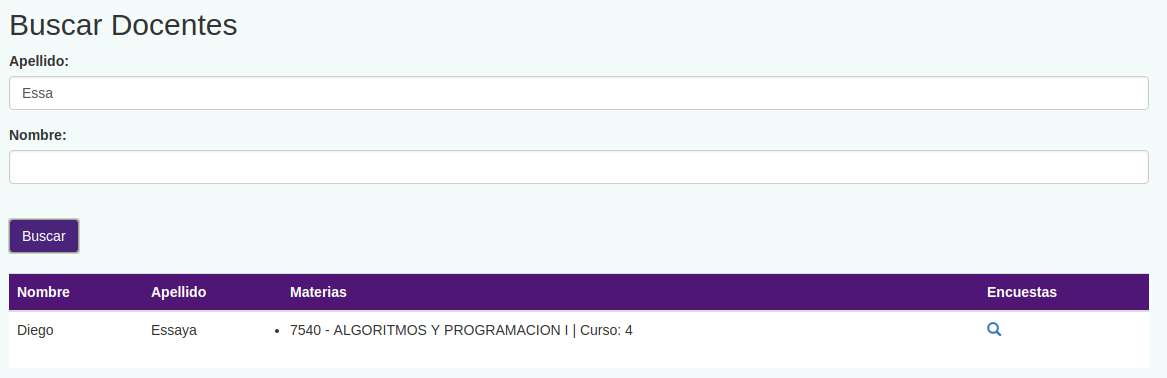
\includegraphics[scale=0.3]{Imagenes/buscar_docentes.png}\par
\caption{Búsqueda de docentes}
\end{figure}

\subsection{Resultados de Encuestas de Docentes}

Para un docente dado, se puede acceder a las encuestas del mismo. Allí, se mostrará el detalle de las materias que dicta con su curso correspondiente y se podrán acceder a las encuestas por cuatrimestre o ver todas reunidas en un mismo lugar.

Ya sea en la visualización por cuatrimestre o en la vista completa, los comentarios realizados al docente se agruparán por curso en que dicta.

\begin{figure}[H]
\centering
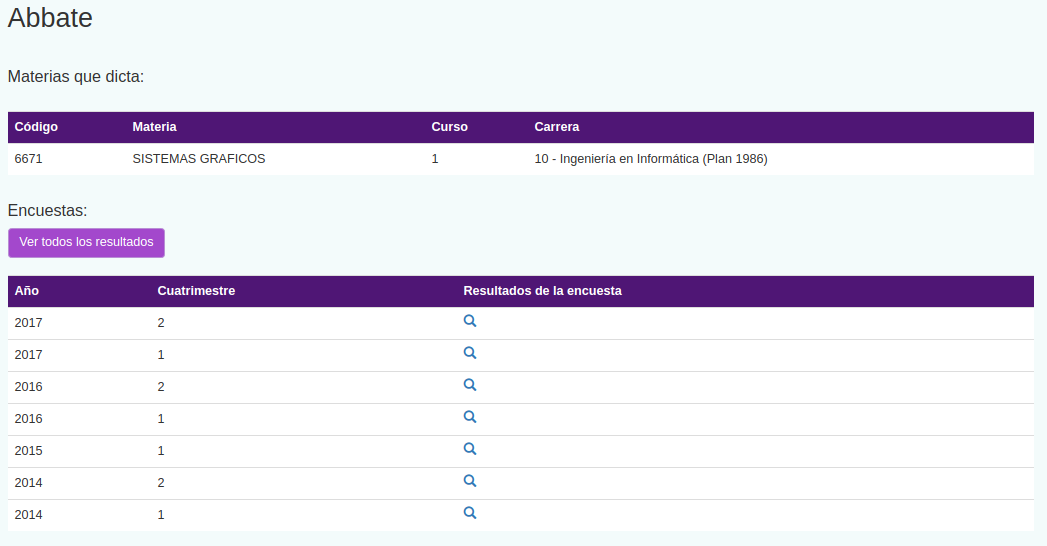
\includegraphics[scale=0.35]{Imagenes/resultados_encuesta_docente.png}\par
\caption{Lista de resultados de encuestas para un docente dado}
\end{figure}

\begin{figure}[H]
\centering
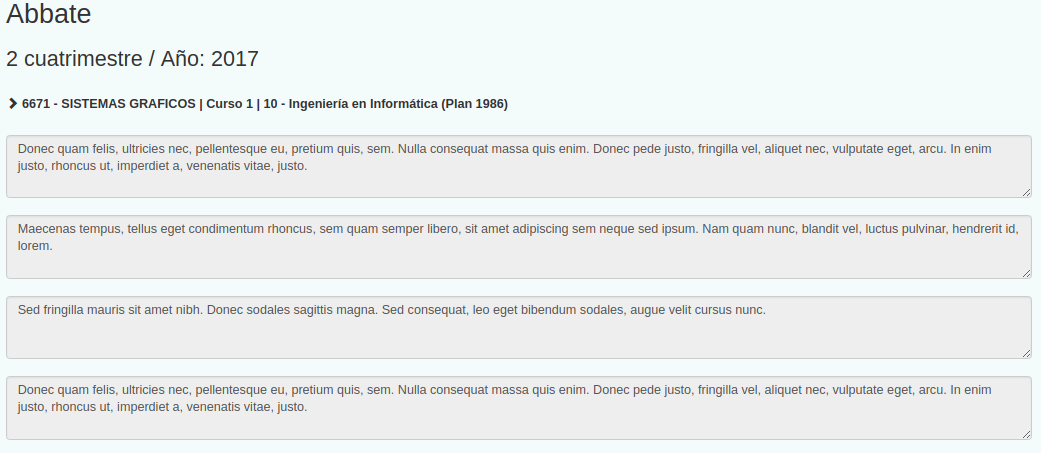
\includegraphics[scale=0.35]{Imagenes/resultados_encuesta_cuatrimestre_docente.png}\par
\caption{Resultados de encuestas docente para un cuatrimestre específico}
\end{figure}

\subsection{Búsqueda de Materias}

La búsqueda de materias se podrá realizar filtrando por los siguientes datos:

\begin{itemize}
	\item Carrera
	\item Código de materia
	\item Nombre (o parte del nombre) de la materia
	\item Palabras clave
\end{itemize}

\begin{figure}[H]
\centering
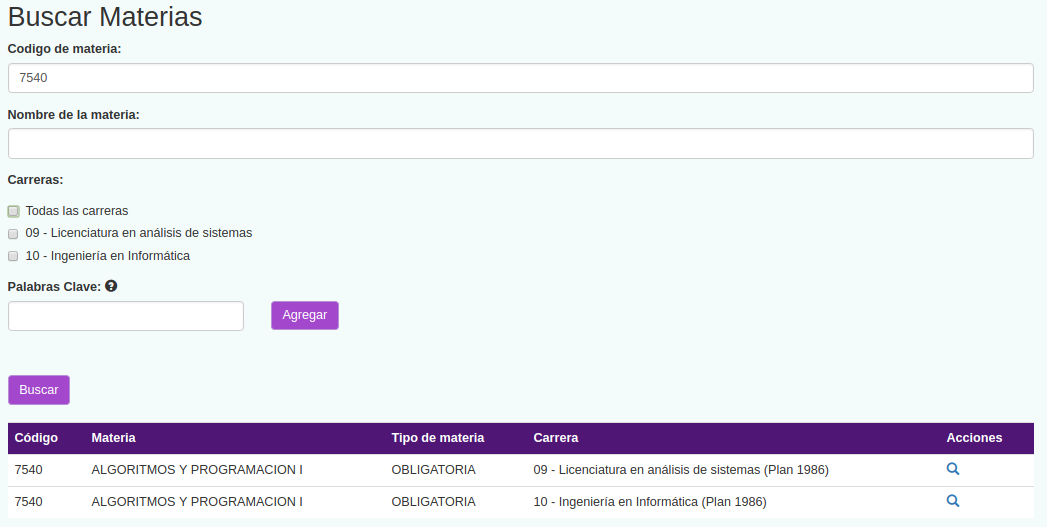
\includegraphics[scale=0.35]{Imagenes/buscar_materias.png}\par
\caption{Búsqueda de Materias}
\end{figure}

Para cada materia se podrán acceder a los datos generales de la misma, en los que se indicará la carrera, la cantidad de créditos, el link a la materia equivalente para otra carrera, las correlativas y el listado de cursos.
En el listado de cursos es posible visualizar el puntaje del mismo (están ordenados por este criterio), y desde allí se puede acceder a los resultados de las encuestas del curso.

\begin{figure}[H]
\centering
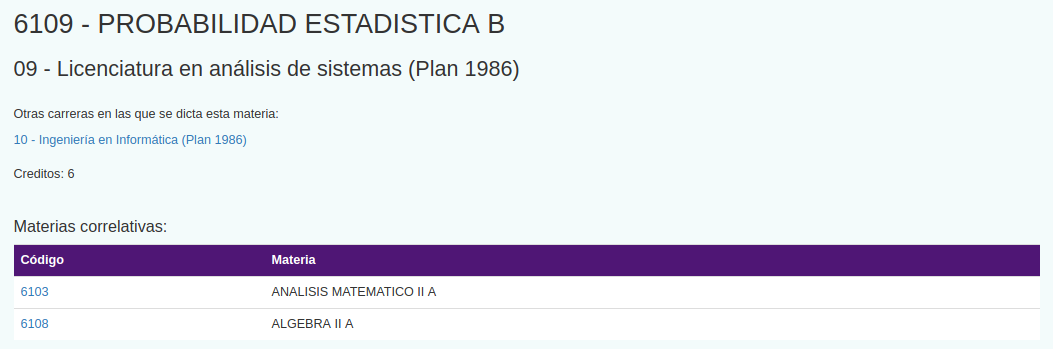
\includegraphics[scale=0.35]{Imagenes/ver_materia_datos_generales.png}\par
\caption{Visualización de una materia}
\end{figure}

\begin{figure}[H]
\centering
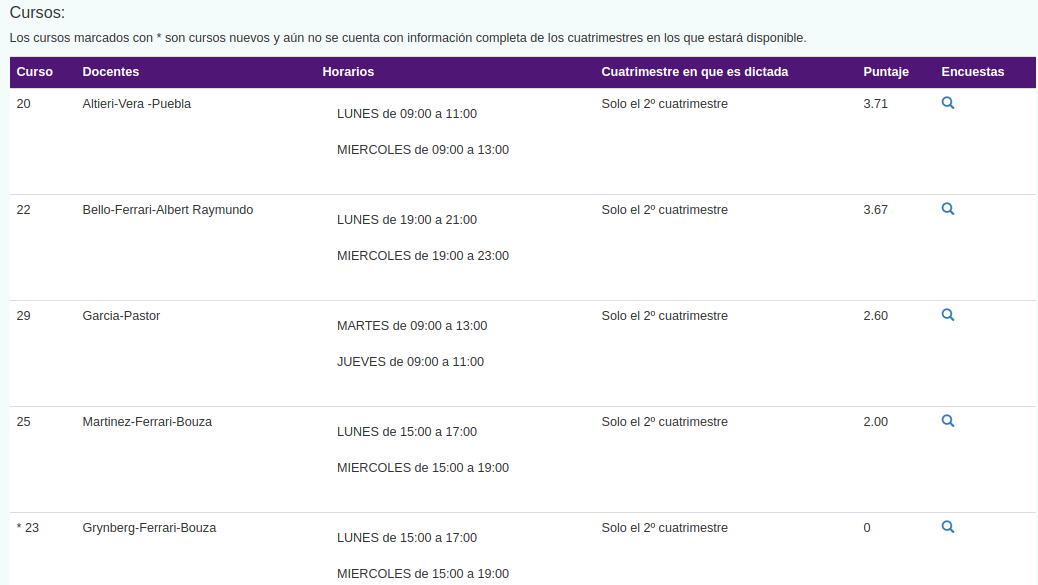
\includegraphics[scale=0.35]{Imagenes/ver_materia_cursos.png}\par
\caption{Cursos de una materia}
\end{figure}

\subsection{Resultados de Encuestas de un curso}

En los resultados de las encuestas de un curso, se pueden visualizar las mismas por cada cuatrimestre para el que haya encuestas finalizadas o como un compilado de todas las respuestas.

\begin{figure}[H]
\centering
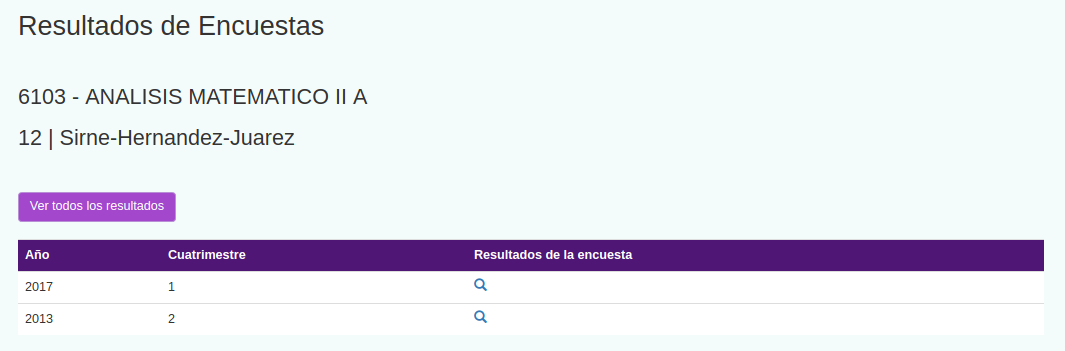
\includegraphics[scale=0.35]{Imagenes/listado_resultados_encuesta_curso.png}\par
\caption{Cursos de una materia}
\end{figure}

Los resultados de las encuestas por curso están divididos en 5 secciones: General, Contenido, Clases, Exámenes y Docentes. Algunas de las respuestas se visualizan como textos, otras como nubes de palabras, otras con gráficos de torta y/o de barras, otras con tablas y otras con mapas de calor. La forma de visualizar los datos dependerá del tipo de pregunta.

\begin{figure}[H]
\centering
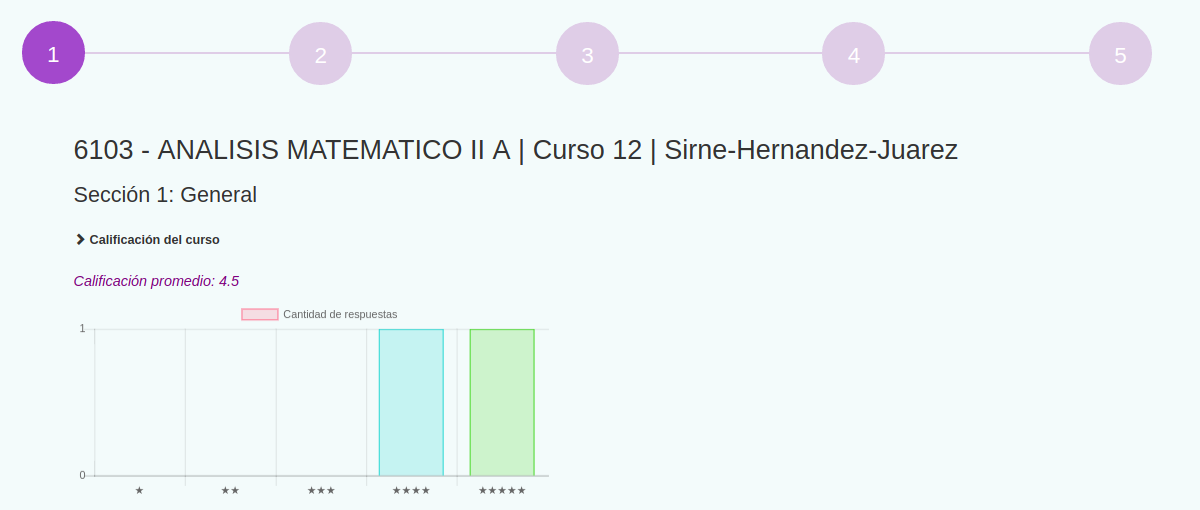
\includegraphics[scale=0.3]{Imagenes/secciones_resultados_encuesta.png}\par
\caption{Secciones de los resultados de la encuesta}
\end{figure}

\begin{figure}[H]
\centering
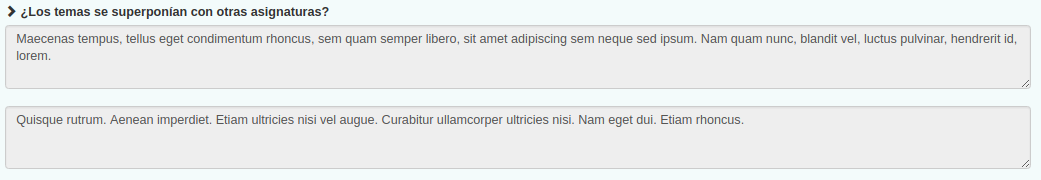
\includegraphics[scale=0.35]{Imagenes/resultados_texto.png}\par
\caption{Ejemplo visualización de resultados de textos}
\end{figure}

\begin{figure}[H]
\centering
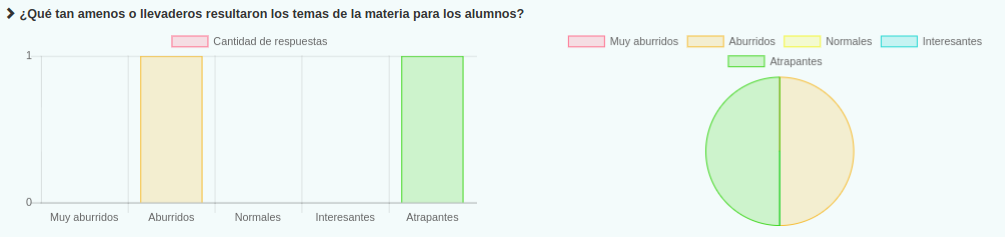
\includegraphics[scale=0.35]{Imagenes/resultados_grafico_torta_y_barras.png}\par
\caption{Ejemplo visualización de resultados con gráfico de torat y de barras}
\end{figure}

\begin{figure}[H]
\centering
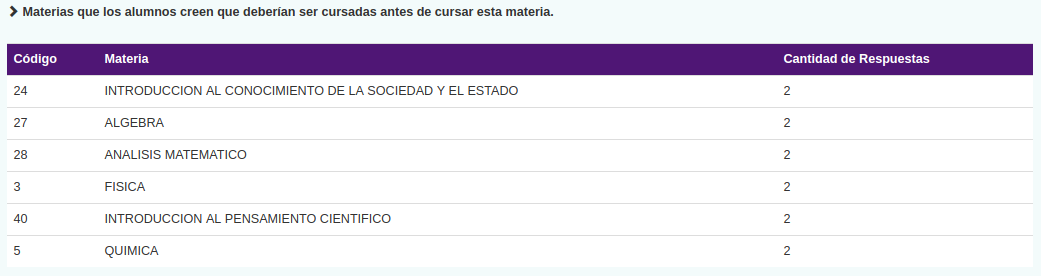
\includegraphics[scale=0.35]{Imagenes/resultados_con_tabla.png}\par
\caption{Ejemplo visualización de resultados con tabla}
\end{figure}

\begin{figure}[H]
\centering
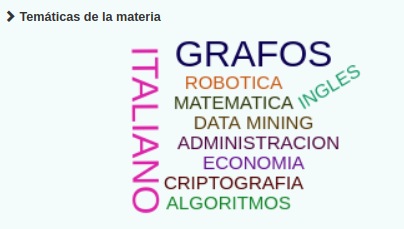
\includegraphics[scale=0.35]{Imagenes/resultados_nubes_de_palabras.png}\par
\caption{Ejemplo visualización de resultados con nubes de palabras}
\end{figure}

\begin{figure}[H]
\centering
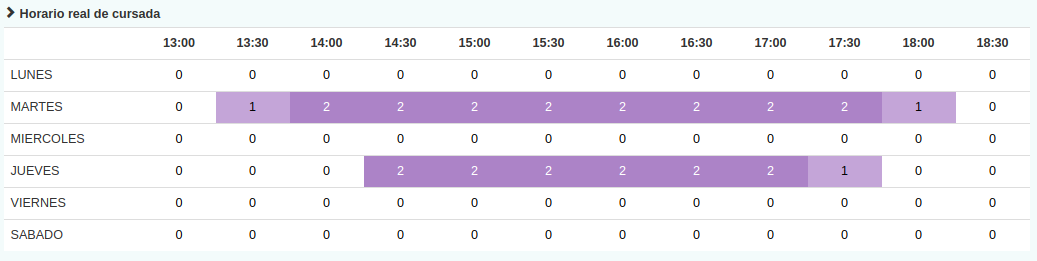
\includegraphics[scale=0.35]{Imagenes/resultados_con_mapa_de_calor.png}\par
\caption{Ejemplo visualización de resultados con mapa de calor}
\end{figure}

\newpage
\section{Página Web MUSSA: Usuarios}

\subsection{Login / Sign In / Cambio de contraseñas}

Tal como se indicó en la sección de herramientas y tecnologías para el dearrollo de esta sección fue utilizado Flask-User y luego customizado el mismo.

Para registrarse es necesario ingresar un e-mail, el nombre, apellido y una contraseña. Esto enviará un email a la diracción indicada para que confirme la registración. Una vez confirmada ya podrá ingresar normalmente al sistema utilizando solamente el e-mail y la contraseña. El padrón no es solicitado en la registración pero se podrá guardar desde los datos académicos, de esta forma los alumnos del CBC podrán hacer uso del sistema incluso antes de tener un padrón asignado.

\begin{figure}[H]
\centering
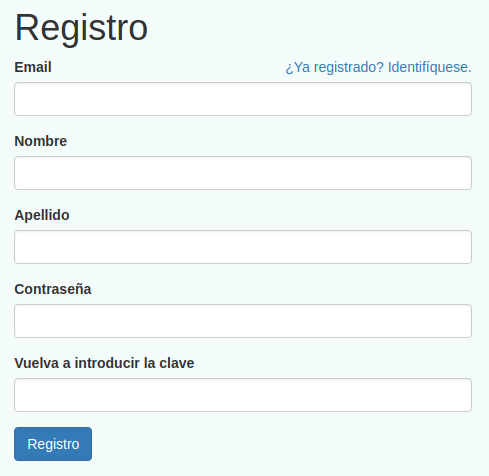
\includegraphics[scale=0.4]{Imagenes/registracion.png}\par
\caption{Registración de usuario}
\end{figure}

\begin{figure}[H]
\centering
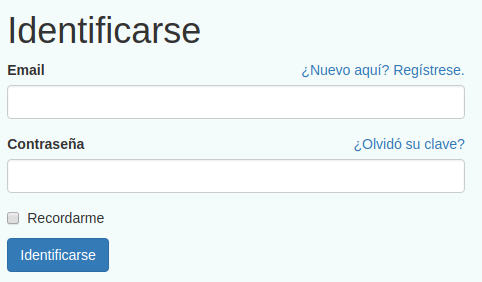
\includegraphics[scale=0.4]{Imagenes/iniciar_sesion.png}\par
\caption{Inicio de sesión}
\end{figure}

En el caso de que el usuario haya olvidado su contraseña podrá ingresar a la sección correspondiente e ingresando el e-mail solicitar el cambio. Solo se le enviará el link de recupero de contraseña al e-mail que esté registrado. En ese e-mail recibirá el link para realizar el cambio de contraseña.
Es posible también cambiar la contraseña una vez ingresado al sistema en caso de que el usuario no la haya olvidado y simplemente desee modificarla desde el perfil del usuario.

\begin{figure}[H]
\centering
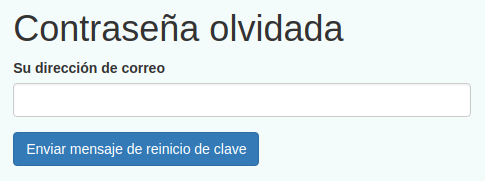
\includegraphics[scale=0.4]{Imagenes/olvido_clave.png}\par
\caption{Recuperar contraseña}
\end{figure}

\subsection{Perfil de usuario}

El usuario registrado podrá modificar su nombre y/o apellido desde su perfil. Se decidió que no se almacenarán otros datos sensibles como el DNI, domicilio o teléfono.\newline

Desde el registro académico el usuario podrá ingresar un padrón (no obligatorio). Si ingresa el padrón, éste debe ser único, es decir que no debe haber otro usuario que ya posea ese padrón.
El alumno podrá registrar la/s carrera/s en la/s que se encuentra inscripto.\newline 

\begin{figure}[H]
\centering
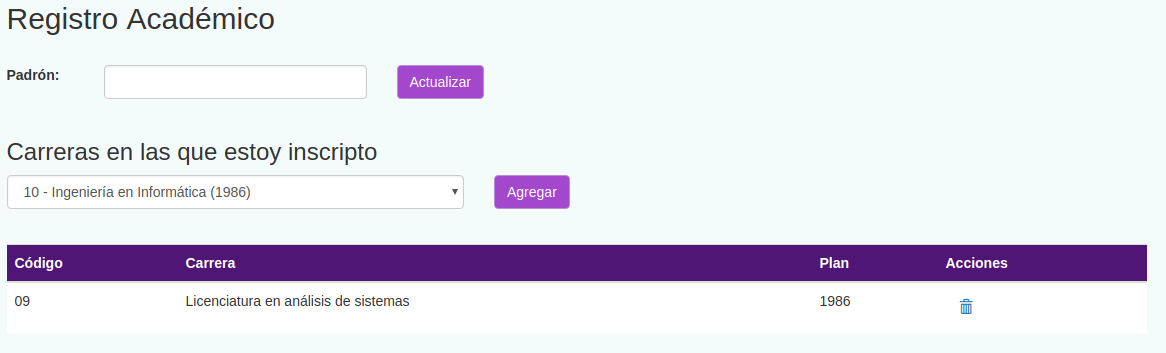
\includegraphics[scale=0.3]{Imagenes/padron_y_carreras.png}\par
\caption{Padrón del alumno y carreras en las que está inscripto}
\end{figure}

Al inscribirse en una carrera, se le habilitarán las materias de la misma para que pueda agregarlas como ''En curso'', ''Con Final Pendiente'', ''Desaprobada'' o ''Aprobada''.Si una materia se desaprueba, entonces se vuelve a habilitar la materia para ser agregada, pero ésta debe tener la cursada en un cuatrimestre posterior (ya que si fue aprobada no se puede volver a cursar).
Al agregar una materia no se hace la verificación de correlativas ya que no se desea restringir la carga, especialmente porque esta versión del proyecto aún no incluye las excepciones de correlatividades.\newline

\begin{figure}[H]
\centering
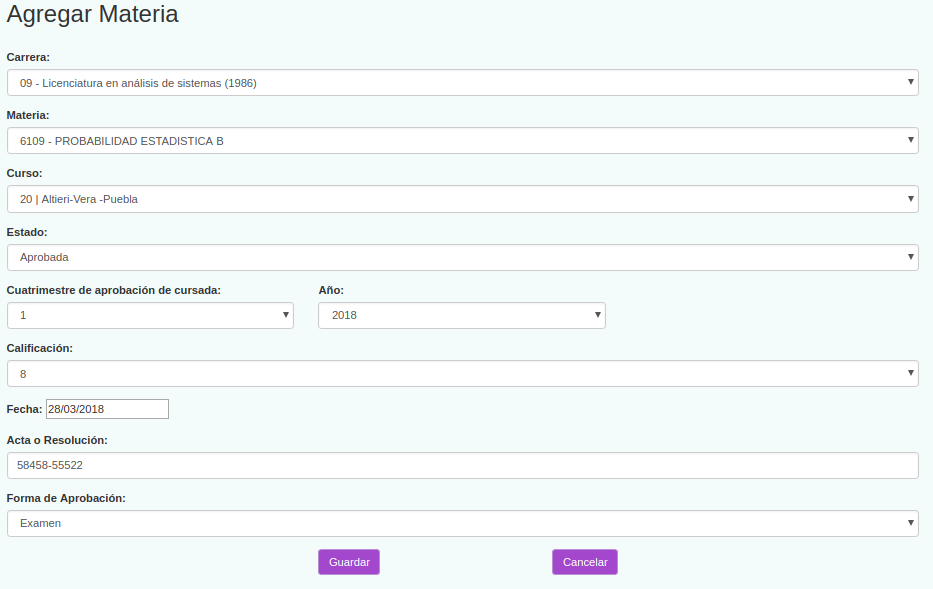
\includegraphics[scale=0.4]{Imagenes/agregar_materia.png}\par
\caption{Agregar Materia Alumno}
\end{figure}

Cuando se carga una materia es posible elegir el curso en el que está siendo cursada / fue cursada dicha materia. En el caso de las materias del CBC no hay cursos disponibles. En el caso de que el curso en el que fue realizada la materia ya no esté disponible (o que el alumno ya no recuerde el curso por algún motivo), es posible indicar que no se seleccionará curso. Cuando la materia no tiene un curso seleccionado no genera entrada de encuesta, ya que cada encuesta está asociado a un curso en particular y no a la materia en general.\newline

La visualización de las materias se puede realizar con las materias de todas las carreras al mismo tiempo, o filtrándolas por carrera. En caso de que se seleccione una carrera en paricular (o solo se esté isncripto a una carrera), se mostrará además el progreso.\newline

\begin{figure}[H]
\centering
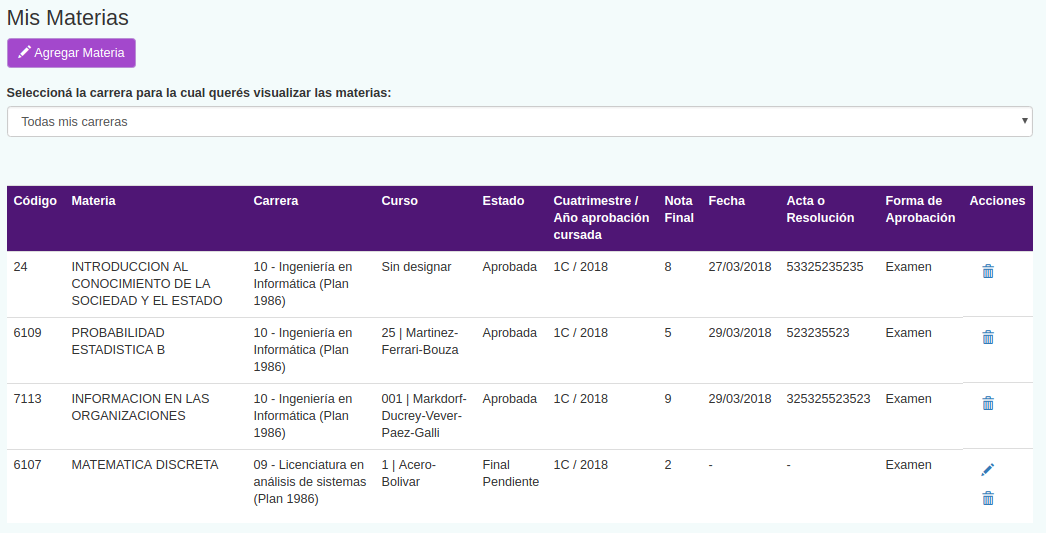
\includegraphics[scale=0.35]{Imagenes/mis_materias_todas.png}\par
\caption{Listado de materias de todas las carreras en las que el alumno está inscripto}
\end{figure}

El progreso indica el porcentaje de avance total de la carrera, el promedio obtenido y el porcentaje de avance en cada uno de los requerimientos de la carrera (cantidad de materias del CBC, créditos en electivas, créditos en materias obligatorias, créditos en materias de orientación (si corresponde), créditos en trabajo final de la carrera (tesis o trabajo profesional si corresponden)).\newline

\begin{figure}[H]
\centering
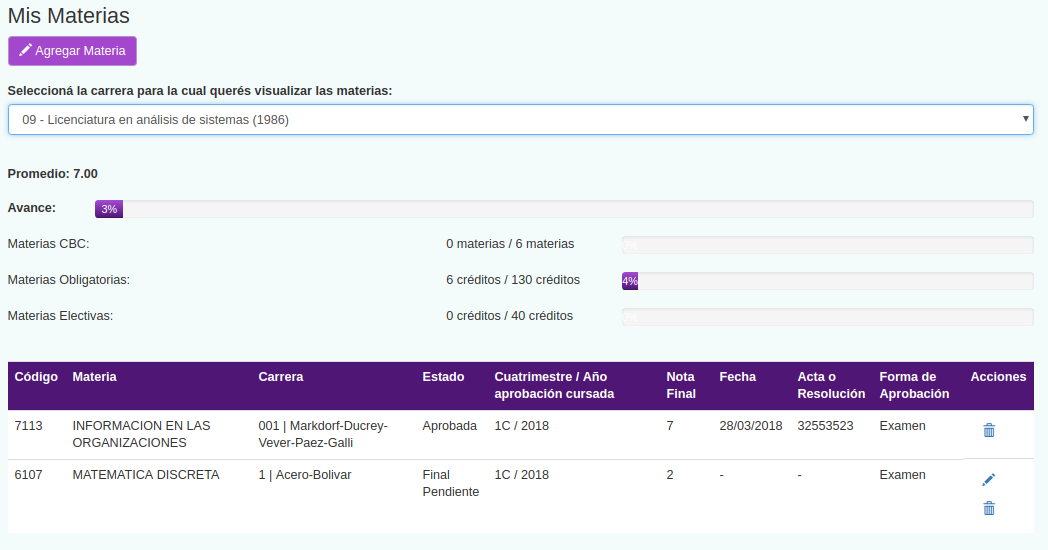
\includegraphics[scale=0.35]{Imagenes/progreso_licenciatura.png}\par
\caption{Progreso y materias filtradas Licenciatura en Análisis de Sistemas}
\end{figure}

\begin{figure}[H]
\centering
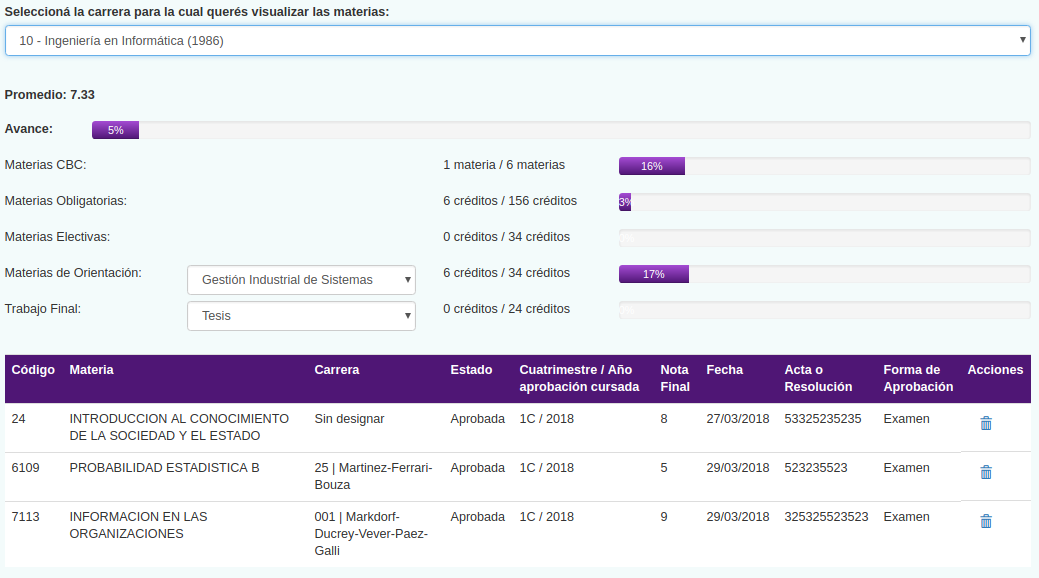
\includegraphics[scale=0.35]{Imagenes/progreso_informatica.png}\par
\caption{Progreso y materias filtradas Ingeniería en Informática}
\end{figure}

\subsection{Materias habilitadas para cursar}

En base a las materias que el alumno tiene ''Aprobadas'' (no incluye las de final pendiente), se mostrará el listado de materias habilitadas para cursar. Como las correlatividades no son transitivas puede suceder que el alumno haya agregado que aprobó Análisis Matemático II pero aún no haya aprobado las materias del CBC, en ese caso se le mostrarán como habilitadas las materias del CBC ya que no poseen ninguna correlativa y todas aquellas materias que sólo hayan tenido a Análisis Matemático II como única correlativa. Posteriormente cuando en futuros desarrollos se agreguen las excepciones de correlatividades, en este punto se mostrarán también aquellas materias que pueden ser cursadas con pedido de excepción ya que se puede decir que estarían ''habilitadas''.

\begin{figure}[H]
\centering
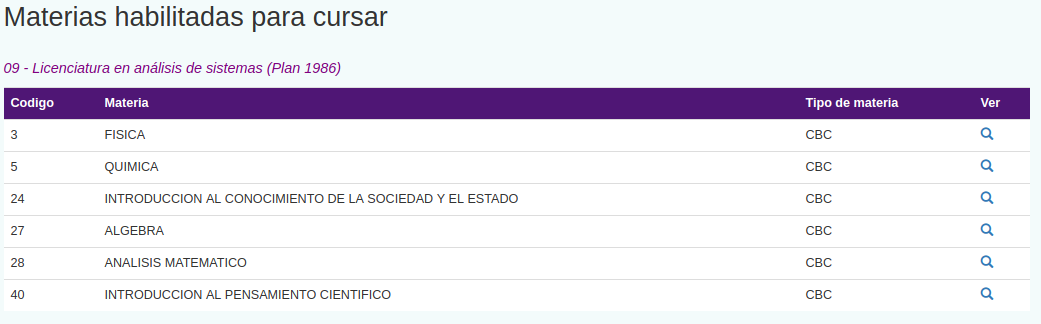
\includegraphics[scale=0.35]{Imagenes/que_puedo_cursar.png}\par
\caption{Listado de materias habilitadas para cursar separados por carrera inscripta}
\end{figure}

\subsection{Formularios}

El alumno puede generar formularios PDF. Los formularios disponibles para esta versión son la nota al decano (formulario más genérico que es solicitado para la mayoría de los trámites) y el listado de materias.

\begin{figure}[H]
\centering
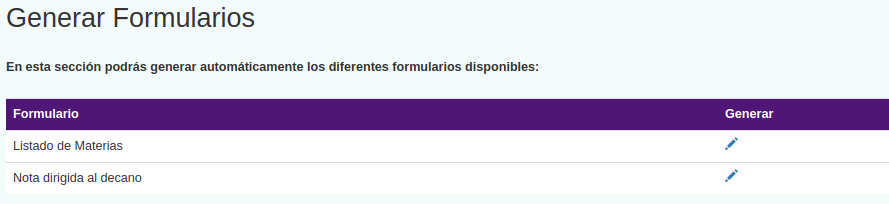
\includegraphics[scale=0.4]{Imagenes/listado_formularios.png}\par
\caption{Formularios disponibles}
\end{figure}

Para el caso del listado de materias se pueden seleccionar las carreras (de las que está inscripto) que desea incluir. Además se debe seleccionar si se desean incluir sólo las materias aprobadas y desaprobadas, las de final pendiente, las que están en curso o más de una de ellas.

\begin{figure}[H]
\centering
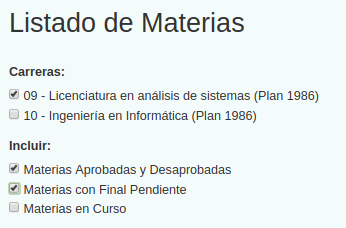
\includegraphics[scale=0.5]{Imagenes/formulario_listado_materias.png}\par
\caption{Configuración formulario listado de materias}
\end{figure}

Para la nota dirigida al decano, se debe establecer el objeto y motivo de la nota. Además se deben indicar los datos personales y de contacto que son solicitados por este modelo. Opcionalmente, se puede ingresar una nota extendiendo los motivos de la solicitud.
Tal como lo solicita el template publicado por la facultad, además de estos datos añadirá el listado de materias aprobadas, desaprobadas, con final pendiente y en curso según corresponda.

\begin{figure}[H]
\centering
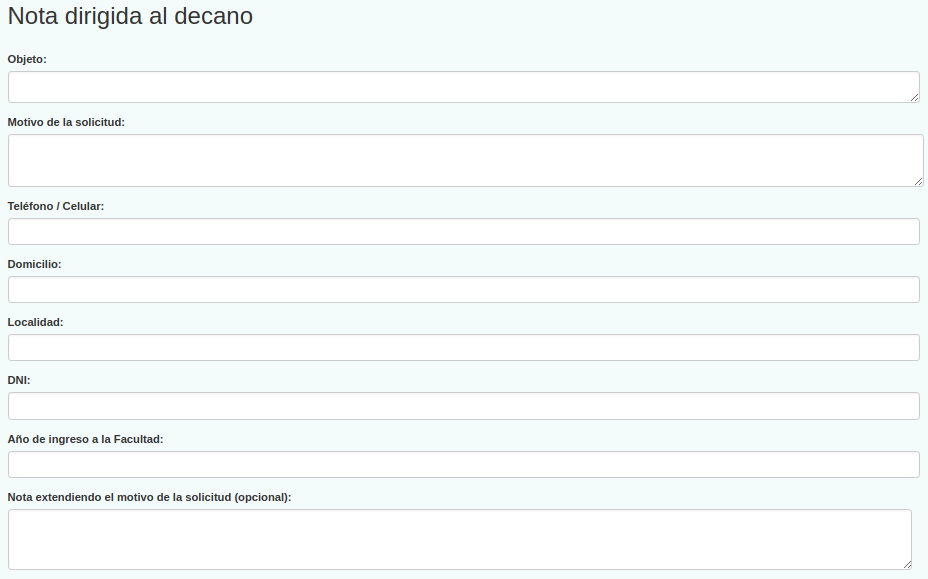
\includegraphics[scale=0.4]{Imagenes/formulario_nota_al_decano.png}\par
\caption{Formulario: Nota dirigida al decano}
\end{figure}

\subsection{Encuestas}

Cuando se agrega una materia con final pendiente, aprobada o desaprobada con un curso específico, se crea una entrada para completar la encuesta correspondiente. Cada alumno tendrá su listado de encuestas realizadas y podrá contestar una sola vez la combinación [curso + cuatrimestre + año] que corresponde a la materia que ha agregado a su historial.

Mientras que haya encuestas pendientes, se mostrará un ícono en el menú correspondiente. Cuando las encuestas pendientes son finalizadas el ícono desaparecerá.

\begin{figure}[H]
\centering
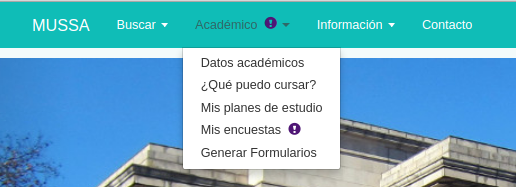
\includegraphics[scale=0.4]{Imagenes/notificacion_encuestas.png}\par
\caption{Notificación de encuestas pendietes}
\end{figure}

En la sección de encuestas se pueden encontrar las encuestas pendientes para ser completadas y visulizar las encuestas que ya fueron finalizadas por el alumno.

\begin{figure}[H]
\centering
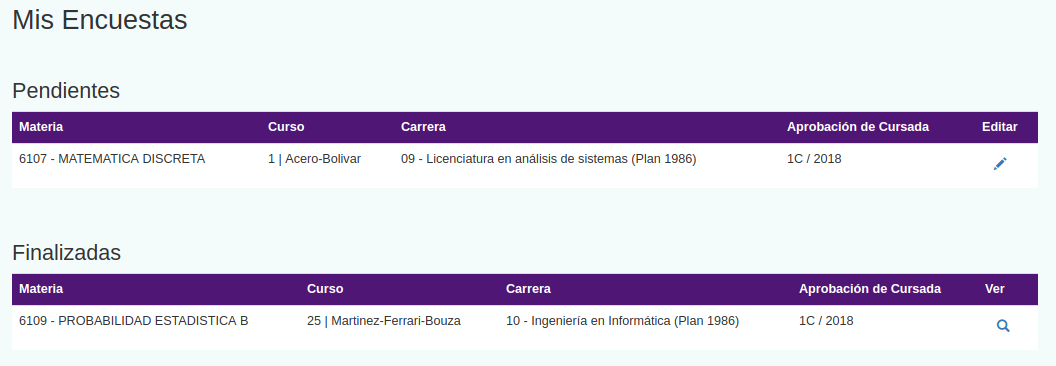
\includegraphics[scale=0.3]{Imagenes/historial_de_encuestas.png}\par
\caption{Historial de encuestas / Encuestas pendientes}
\end{figure}

Cada encuesta a completar cuenta con preguntas en 5 secciones: General, Contenido, Clases, Exámenes y Docentes. Cada una de las secciones es guardada de forma parcial de forma que se pueda comenzar con la encuesta en un momento y continuarla más adelante. Una vez que la encuesta se finaliza (y se la guarda como tal) ya no podrá ser editada.

Las preguntas de las encuestas incluyen el puntaje del curso, horario real de cursada, dificultad de los temas, régimen de aprobación, comentarios de los docentes, etc.

Se incluye también una pregunta para indicar la temática de la materia (que será utilizada para clasificar las materias electivas en la generación del plan de carrera) y palabras clave (que son utilizadas en la búsqueda de materias).

\begin{figure}[H]
\centering
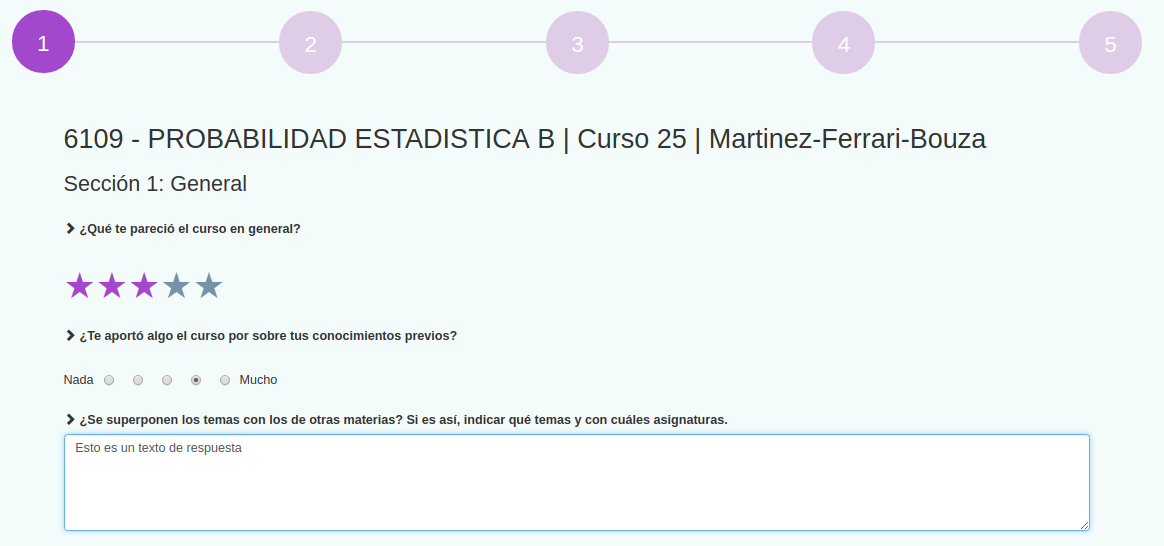
\includegraphics[scale=0.3]{Imagenes/completar_encuesta.png}\par
\caption{Encuesta para completar}
\end{figure}

La encuesta ha sido modelada como un set de preguntas, donde cada pregunta puede ser de un tipo diferente y conforme a ello será la manera en que será renderizada en la web. Entre los tipos de preguntas se encuentran las de texto, horarios, correlativas, números, estrellas, puntaje, entre otras.\newline

Los resultados de las encuestas que se pueden ver también desde el modo público, solo incluyen las encuestas que ya han sido finalizadas.

\subsection{Generación y Visualización del Plan de Carrera}

Para permitir el armado del plan, se deberán poder establecer las preferencias del alumno. Las preferencias básicas que pueden elegirse son:

\begin{itemize}
	\item Carrera (Orientación y Trabajo Final de Carrera si corresponde)
	\item Máxima cantidad de materias por cuatrimestre
	\item Horarios en los que el alumno no puede cursar
	\item Cursos específicos en los que el alumno quiera cursar (puede elegir uno, niguno o varios cursos). Se elige el curso pero no en qué cuatrimestre éste será cursado.
\end{itemize}

Además, en caso de tener materias con final pendiente, se deberá indicar cuándo se puede considerar la materia como aprobada, de forma tal que se restrinja el cuatrimestre mínimo de las materias que la tienen como correlativa.

\begin{figure}[H]
\centering
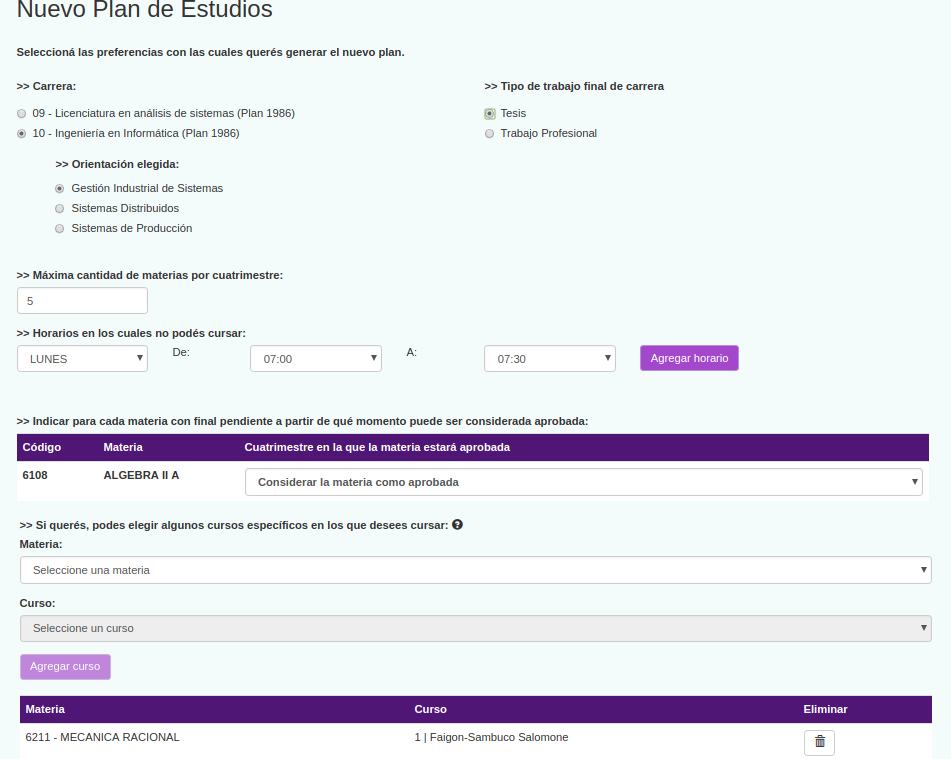
\includegraphics[scale=0.35]{Imagenes/preferencias_generacion_plan.png}\par
\caption{Preferencias para generación del plan de estudios}
\end{figure}

Adicionalmente, se podrán establecer las siguientes opciones avanzadas:

\begin{itemize}
	\item Algoritmo de generación del plan: PLE (Programación Lineal Entera) o Greedy
	\item Máxima cantidad de cuatrimestres de duración del plan (el algoritmo siempre tratará de minimizarlos)
	\item Puntaje mínimo requerido para los cursos: Los cursos no puntuados tienen un puntaje de 0. La restricción de puntaje no es tenida en cuenta en el caso de los cursos que se seleccionan manualmente. Las materias que se elijan no tendrán un puntaje menor al seleccionado a menos que sean obligatorias con un único curso disponible. En estos casos siempre se seleccionará en orden la de mayor puntaje con mayor cantidad de encuestas completas.
	\item Máxima cantidad de horas de cursada, por semana
	\item Máxima cantidad de horas de trabajo extra además de la cursada, por semana
	\item Cuatrimestre y Año de inicio del plan (se selecciona el cuatrimestre y año actual por defecto). Este dato es importante no solo para la visualización sino también porque hay algunas materias que solo se dictan el 1º o 2º cuatrimestre.
	\item Preferencias de temáticas de las materias electivas: El porcentaje indicado será el porcentaje mínimo de cada temática respecto del total de créditos en electivas restantes que debe realizarse. Si una materia tiene más de una temática elegida, sus créditos serán contandos para ambos porcentajes.
\end{itemize}

\begin{figure}[H]
\centering
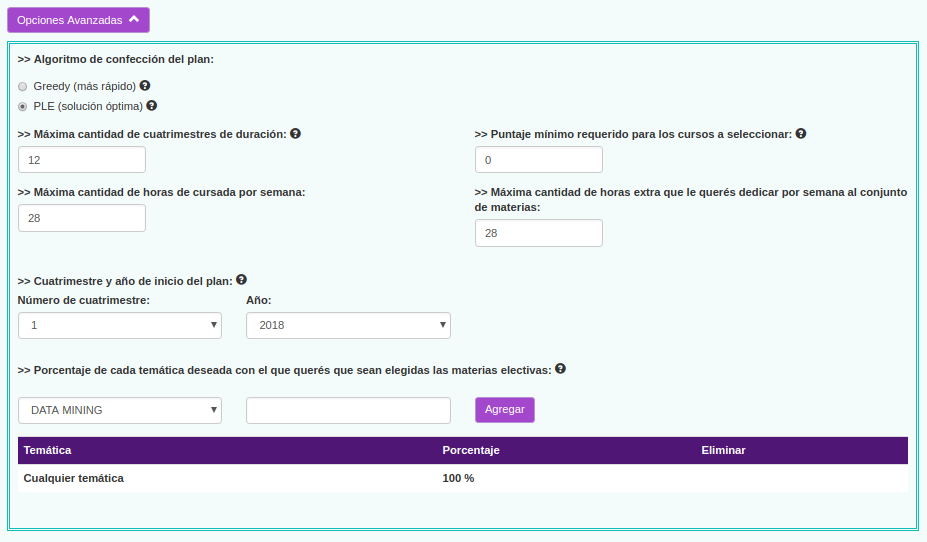
\includegraphics[scale=0.35]{Imagenes/preferencias_avanzadas_generacion_plan.png}\par
\caption{Preferencias Avanzadas para generación del plan de estudios}
\end{figure}

Cuando el plan esté generado, se mostrará una notificación en el menú.

\begin{figure}[H]
\centering
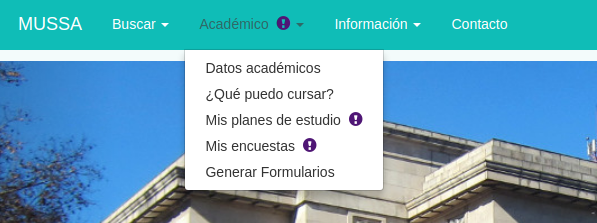
\includegraphics[scale=0.35]{Imagenes/notificacion_plan_generado.png}\par
\caption{Notificación Plan Generado no visualizado}
\end{figure}

Es posible visualizar el listado de los planes de estudio que se han solicitado. Cada uno de ellos tendrá el estado 'En curso' (aún se está generando o está en la cola de espera), 'Incompatible' (no hay una solución óptima que cumpla con los parámetros indicados) o 'Finalizado' (plan compatible finalizado de generar).

\begin{figure}[H]
\centering
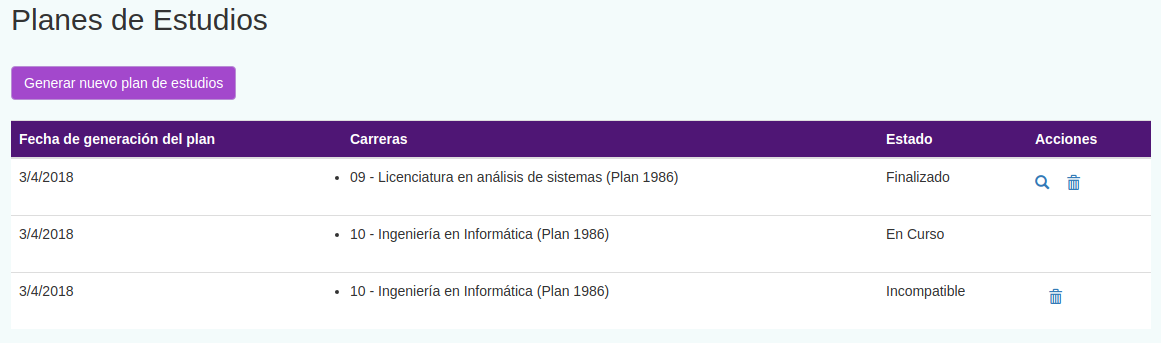
\includegraphics[scale=0.3]{Imagenes/historial_planes_generados.png}\par
\caption{Historial Planes Generados}
\end{figure}

Los planes que se encuentren en estado 'Finalizado' o 'Incompatible' se los podrá eliminar.

Los planes que se encuentren en estado 'Finalizado' pueden ser visualizados.

La visualización del plan de estudios consiste en el listado de los cuatrimestres con las materias para cada uno de ellos. En el caso de que se hayan cargado materias que no hayan sido contempladas en el momento de la generación del plan, éstas serán agregadas en el cuatrimestre correspondiente y eliminadas del asignado originalmente (si corresponde).

Las materias con estados diferentes se mostrarán con otros colores para facilitar la diferenciación entre ellas.

\begin{figure}[H]
\centering
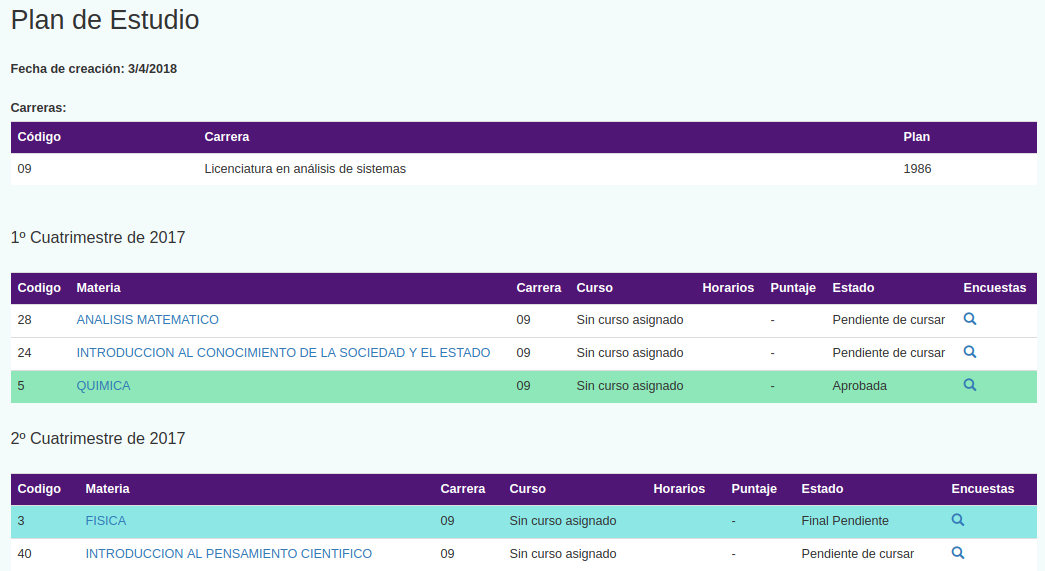
\includegraphics[scale=0.35]{Imagenes/vista_plan_generado.png}\par
\caption{Visualización Plan Generado}
\end{figure}

\newpage
\section{Página Web MUSSA: Acceso Administrador}

El usuario con rol de administrador tiene habilitado un menú de Administración para los horarios, los cursos y los docentes.

\subsection{Administrar Horarios}

Los horarios y los cursos son cargados al sistema a través del PDF que es publicado por la Facultad todos los cuatrimestres. Esta es la única fuente de datos disponible desde la facultad para obtener los datos de los horarios completos, ya que la otra opción implica parsear una página web desde el sistema SIU Guaraní.

Cuando se carga el PDF se verifica que los horarios que se están cargando no se hayan cargado antes y que el cuatrimestre y año sea superior al último que se cargó (para que no se carguen horarios viejos modificando los datos actuales).

\begin{figure}[H]
\centering
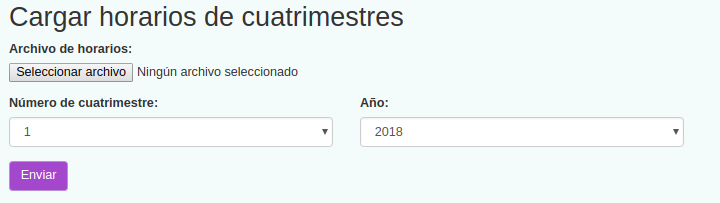
\includegraphics[scale=0.35]{Imagenes/administrar_horarios.png}\par
\caption{Carga de Horarios PDF}
\end{figure}

Al principio se consultó con la facultad para poder tener un servicio y obtener estos datos (entre otros) y se tuvo una respuesta negativa.

El problema con este mecanismo es que el PDF la facultad lo publica y suele contener muchos errores que son corregidos conforme pasan las semanas en el SIU Guaraní, pero no se vuelve a publicar el archivo, por lo que los horarios erróneos deben modificarse manualmente con la administración de cursos. En versiones futuras, se desea agregar a los alumnos la opción de reportar cursos con datos incorrectos de forma de que se simplifique la tarea del administrador.

Debido a estos errores, lo ideal es utilizar el PDF actual como carga inicial y luego facilitar un administrador con un nuevo rol habilitado para cada departamento, de forma que cada departamento pueda hacer los cambios de los cursos que se han cambiado solo ese cuatrimestre y no de todos. Es ideal que los departamentos luego quieran utilizar el sistema, ya que podrían hacer uso de las encuestas para monitorizar los cursos correspondientes y poder hablar con los docentes ya sea para felicitarlos o para solicitarles que realicen ajustes en sus materias.

Otro problema que se tiene con el PDF es que los docentes que figuran en los cursos no son todos los que el curso realmente tiene, por lo que habría que agregar el resto del equipo docente manualmente si se quiere poder tener encuestas de ellos. Además, la única referencia al docente es su apellido, por lo que no es posible saber si el docente con apellido X que da la materia M1 es el mismo (o no) que el docente con apellido X que dicta la materia M2. Este link de docentes debe realizarse manualmente desde la administración de docentes.

\subsection{Administrar Cursos}

En la administración de cursos es posible visualizar y buscar los cursos por código de materia; ver los docentes que lo dictan, las carreras para las cuales está habilitado y en qué cuatrimestre se dicta.

\begin{figure}[H]
\centering
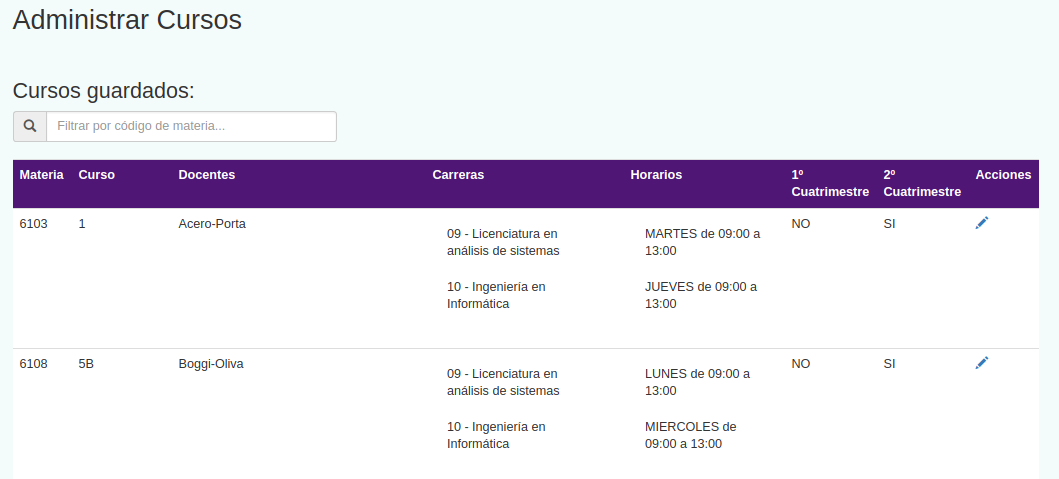
\includegraphics[scale=0.3]{Imagenes/administrar_cursos.png}\par
\caption{Administración de Cursos}
\end{figure}

Cuando se cargan los horarios PDF de un cuatrimestre, se dan de alta todos aquellos cursos nuevos (un curso es nuevo si el código/número de curso no existe para ese código de materia) y se marca como que se dicta ambos cuatrimestres, pero que es curso nuevo, registrando el cuatrimestre que fue actualizado (el 1º o el 2º). El curso seguirá siendo nuevo hasta que esté registrado en ambos cuatrimestres. Que esté registrado no quiere decir que se dicte en ambos, sino que se cargaron horarios tanto del 1º cuatrimestre como del 2º desde que el curso se dio de alta.

Si el curso ya existía, entonces se actualiza la lista de docentes y los horarios en los que es dictada la materia.

Al editar un curso, es posible modificar las carreras para las cuales está habilitado, agregar o quitar docentes del curso y modificar los horarios del mismo.

\begin{figure}[H]
\centering
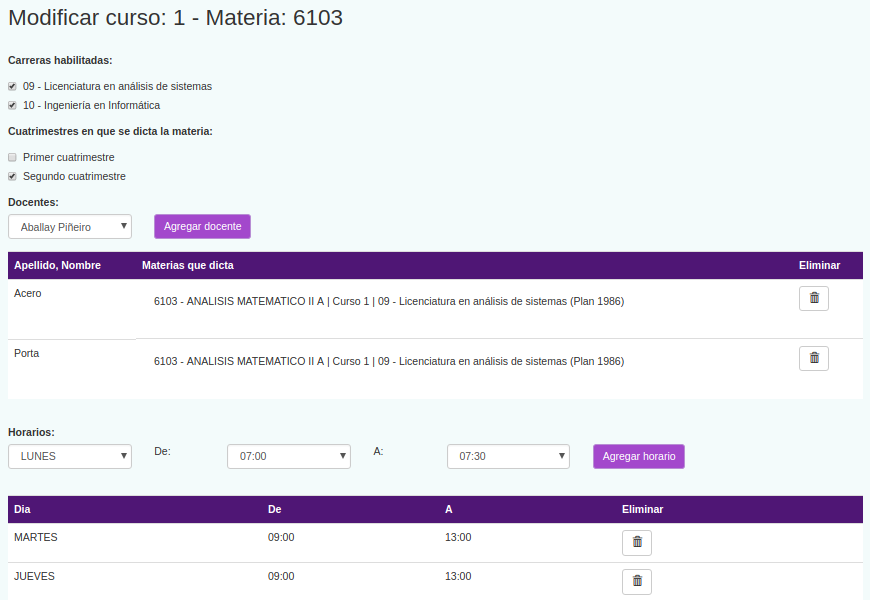
\includegraphics[scale=0.35]{Imagenes/modificar_curso.png}\par
\caption{Edición de un curso}
\end{figure}

\subsection{Administrar Docentes}

En la administración de docentes, es posible agrupar los docentes que se seleccionen. El agrupamiento sólo se permite si todos los docentes a agrupar tienen mismo apellido y nombre (o no tienen nombre). De esta forma, es posible solucionar el problema del docente con apellido X que dicta la materia M1 y otro docente con apellido X que dicta la materia M2, siempre que el administrador posea este conocimeinto.

\begin{figure}[H]
\centering
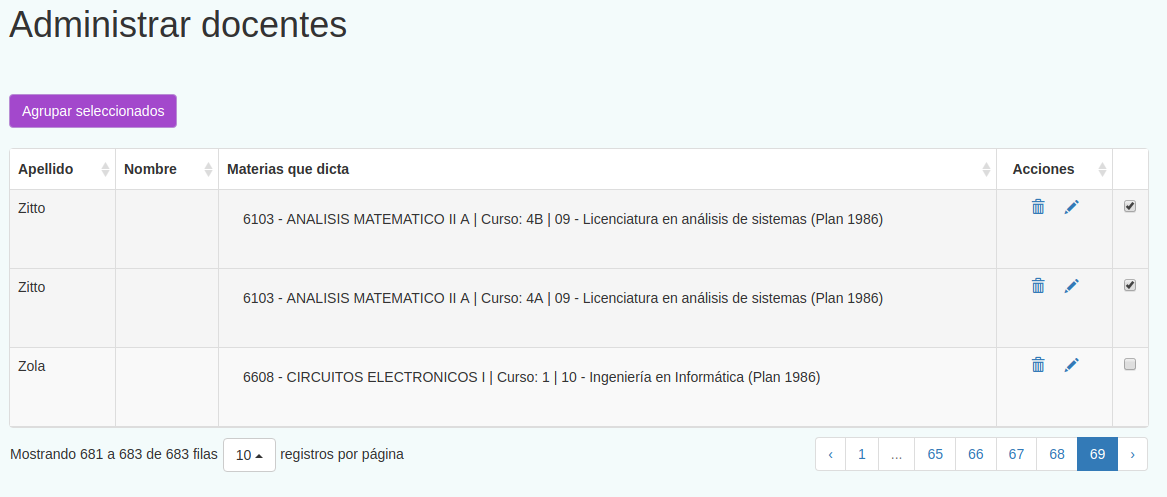
\includegraphics[scale=0.3]{Imagenes/administrar_docentes.png}\par
\caption{Administración de Docentes}
\end{figure}

Al editar un docente, es posible cambiar su nombre, apellido, y cursos que dicta. Se debe tener especial cuidado en que la modificación de estos, como el nombre y el apellido, ya que las encuestas que estén vinculadas a este id docente seguirán estando vinculadas pero mostrarán un nombre diferente del que mostraban originalmente (mostrarán el nombre actualizado). Estos cambios deben realizarse sólo en caso de errores de escritura o de falta de datos y no para modificar un docente por otro.

\begin{figure}[H]
\centering
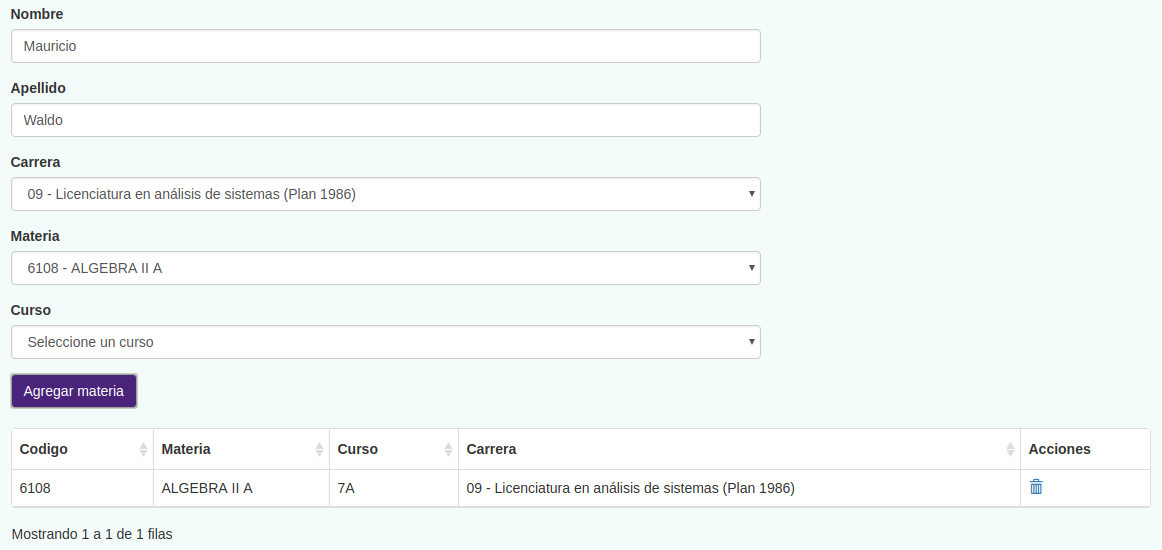
\includegraphics[scale=0.3]{Imagenes/editar_docente.png}\par
\caption{Edición de un Docente}
\end{figure}

\newpage
\section{Algoritmos para la generación del Plan de Estudios personalizado}

\subsection{Arquitectura y Flujo General}
---------------------- HACER -------------------------

\subsection{Configuración de Parámetros}
---------------------- HACER -------------------------

\subsection{Algoritmo Programación Lineal Entera (PLE)}
---------------------- HACER -------------------------

\subsection{Algoritmo Greddy}
---------------------- HACER -------------------------

\subsection{Pruebas}
---------------------- HACER -------------------------


\newpage
\section{Mejoras futuras}

---------------------- HACER -------------------------

\newpage
\section{Conclusiones}

---------------------- HACER -------------------------

\newpage
\section{Agradecimientos}

A mi familia, que estuvo presente desde la distancia cuando comencé la carrera. A mi hermana Lorena que me trajo a Buenos Aires cuando comencé a estudiar en la universidad manejando ambas por la ruta durante esos 2000 kilómetros. A mi hermana Verónica que muchas veces vino a Buenos Aires a visitarme a pesar de que estábamos tan lejos.

A mi nueva familia adquirida, que me han acompañado durante este último tramo, en especial a Nico que nos hizo mil y un favores relacionados a la facultad desde que nos mudamos a Irlanda.

A mis amigos y compañeros de facultad, con los que siempre compartí muy buenas experiencias y muchas veces tuvimos que dejar cosas de lado porque 'había que estudiar'. En especial a Nicolás, Martín, Ezequiel, Flor y Javier con los que compartí la mayor parte de mi carrera y nos ayudamos mutuamente a avanzar, sé muy bien que sin ellos la carrera no hubiese sido igual.

A todos mis grupos de trabajo profesional antes de este, que se armaron y desarmaron por uno u otro motivo, pero que han sido pasos necesarios para poder finalmente llegar a este punto.

A mis tutores, Rosita y Diego que me acompañaron durante este trabajo. En especial a Diego que siendo su primer tutoría me acompañó y me alentó mucho con sus comentarios y recomendaciones.

A todos los Wachencholdiers los que están y los que estuvieron. Con ustedes compartí miles de experiencias y locuras. Aprendí mucho, me divertí mucho. Me sentí muy acompañada y todos los días los extraño un poco. Estoy orgullosa de haber podido ser parte de este gran equipo, y aún me considero parte aunque ya no pueda estar tan cerca...

A mis alumnos, que me enseñaron a enseñar, a tener paciencia, a tener mejor predisposición y a encontrar mil y un maneras de decir lo mismo. Muchas veces siento que las cosas las aprendí realmente al tener que explicarlas a ustedes.

Y de manera especial, agradezco a mi marido, Ariel Wainer, que ha estado conmigo todo este tiempo, sosteniendome en mis tristezas y compartiendo conmigo mis alegrías. Gracias por haberme mostrado tantas herramientas nuevas y por retarme cuando hacía las cosas mal para que las mejorara, sé que no soy fácil pero me encanta que me enseñes y expliques lo que vos sabes. Esto no hubiese sido posible sin vos.


\newpage
\section{Referencias y Material consultado}

\renewcommand\refname{\small}

\begin{thebibliography}{X}

%Formato: Articulos con DOI asignado:

% Autor(es): apellido(s) e inicial del nombre. Sólo considerar los dos apellidos si son de origen español y están %indicados en el documento a citar 
% Año de publicación entre paréntesis, seguido de punto
% Título del artículo, seguido de punto
% Título de la revista en letra cursiva, seguido de coma

% Volumen en letra cursiva y número entre paréntesis (si está mencionado, sin cursiva), seguido de coma

% Números de páginas de inicio y final, separadas por un guión, seguidos de punto

% Coloca la expresión http://dx.doi.org/ y a continuación el número DOI asignado (ver APA Style Guide to Electronic  References - American Psychological Association, pág. 12)

% Articulos sin DOI asignado

% Autor(es): apellido(s) e inicial del nombre. Sólo considerar los dos apellidos si son de origen español y están indicados en el documento a citar 

% Año de publicación entre paréntesis, seguido de punto

% Título del artículo, seguido de punto

%Título de la revista en letra cursiva, seguido de coma

% Volumen en letra cursiva y número entre paréntesis (si está mencionado, sin cursiva), seguido de coma

% Números de páginas de inicio y final, separadas por un guión, seguidos de punto

% Coloca la expresión Recuperado de, seguida de la dirección electrónica (URL) de la página principal de la revista


% BEGIN Referencia
\bibitem{PLE_HORARIOS_UNIV} Rodrigo Hernandez, Jaime Miranda P. y Pablo A. Rey (2008). Programación de Horarios de Clases y Asignación de Salas para la Facultad de Ingeniería de la Universidad Diego Portales Mediante un Enfoque de Programacion Entera. \textit{Revista Ingeniería de Sistemas}, \textit{Volumen XXII}, páginas 121-141.
Recuperado de: \url{http://www.dii.uchile.cl/ris/RISXXII/horariosUDP_RISVersion%20FINAL.pdf}
% END Referencia


% BEGIN Referencia
\bibitem{MODELOS_PLE}
Enrique Castillo, Antonio J. Conejo, Pablo Pedregal, Ricardo García y Natalia Alguacil (2002). Formulación y Resolución de Modelos de Programación Matemática en Ingeniería y Ciencia. Páginas 461-483.
Recuperado de: \url{http://www.dia.fi.upm.es/~jafernan/teaching/operational-research/LibroCompleto}
% END Referencia


% BEGIN Referencia
\bibitem{PAPER_ROSITA_PLANNING_WITH_PREFERENCES_1}
Jorge A. Baier y Sheila A. McIlraith (2008). Planning with Preferences. \textit{Association for the Advancement of Artificial Intelligence}, \textit{Volumen 29 (4)}, páginas 25-36.
\url{https://doi.org/10.1609/aimag.v29i4.2204}
% END Referencia


% BEGIN Referencia
\bibitem{PAPER_ROSITA_PLANNING_WITH_PREFERENCES_2}Shirin Sohrabi, Jorge A. Baier y Sheila A. McIlraith (2009). HTN Planning with Preferences. \textit{Proceedings of the 21st international jont conference on Artifical intelligence},  páginas 1790-1797.
Recuperado de: \url{https://www.ijcai.org/Proceedings/09/Papers/298.pdf}
% END Referencia


% BEGIN Referencia
\bibitem{PAPER_ROSITA_PLANNING_WITH_PREFERENCES_3} Nan Li, William Cushing, Subbarao Kambhampati y Sungwook Yoon (2014). Learning Probabilistic Hierarchical Task Networks as Probabilistic Context-Free Grammars to Capture User Preferences. \textit{ACM Transactions on Computational Logic}, \textit{Volumen V}, páginas 1-32.
Recuperado de: \url{http://rakaposhi.eas.asu.edu/nan-tist.pdf}
% END Referencia


% BEGIN Referencia
\bibitem{PAPER_ROSITA_PLANNING_WITH_PREFERENCES_4} Nan Li, William Cushing, Subbarao Kambhampati y Sungwook Yoon (2013). Learning Probabilistic Hierarchical Task Networks to Capture User Preferences \textit{Preprint submitted to Artificial Intelligence}, páginas 1-30.
Recuperado de: \url{https://arxiv.org/pdf/1006.0274.pdf}
% END Referencia


% BEGIN Referencia
\bibitem{PULP_PYTHON} \textit{<<Linear Programming with Python and PuLP>>}

\textsc{Ben Alex Keen}

\url{http://benalexkeen.com/linear-programming-with-python-and-pulp/}
% END Referencia


% BEGIN Referencia
\bibitem{PULP_DOC_OFICIAL_PYTHON} \textit{<<Optimization with PuLP>>}

\textsc{Stuart Mitchell, Anita Kean, Andrew Mason, Michael O’Sullivan, Antony Phillips}

\url{https://pythonhosted.org/PuLP/}
% END Referencia


% BEGIN Referencia
\bibitem{FLASK_TUTORIAL} \textit{<<The Flask Mega-Tutorial>>}

\textsc{Miguel Grinberg}

\url{https://blog.miguelgrinberg.com/post/the-flask-mega-tutorial-part-i-hello-world}
% END Referencia


\end{thebibliography}

\end{document}